\subsection{Strømforsyning}\label{sec:hwd_psu}

Bilen er udstyret med en strømforsyningen, som har til formål at forsyne hele bilen med strøm ved hhv. 7.2V, 5V og 3V. 
Den komplette beskrivelse af strømforsyningen i sit nuværende stadie kan ses i afsnit \ref{P-sec:car_psu} \nameref{P-sec:car_psu} på side \pageref{P-sec:car_psu} i dokumentationen.
Bilens strømforsyning er designet ud fra princippet om en buck converter\cite[s. 326] {lib:analogteknik}, men med modifikationer således at der udover en 5V udgang også drives en 3V udgang fra samme converter.
De 7.2V leveres direkte fra batteriet og bruges udelukkende til at drive motoren på bilen med.

Designfasen for bilens strømforsyning startede med en simpel håndtegning af en buck converter med både 3 og 5V udgang som havde egen indbygget regulering. 
Grunden til at reguleringen af converteren er så vigtig på denne platform er at batterispændingen nemt kan flytte sige 1-2V eller mere, hvilket overføres direkte til udgangen ved en konstant pulsbredde på styresignalet til switchen. Den oprindelige tegning ses i figur \ref{fig:bil_psu_sketch}.

\begin{figure}[h]
\centering
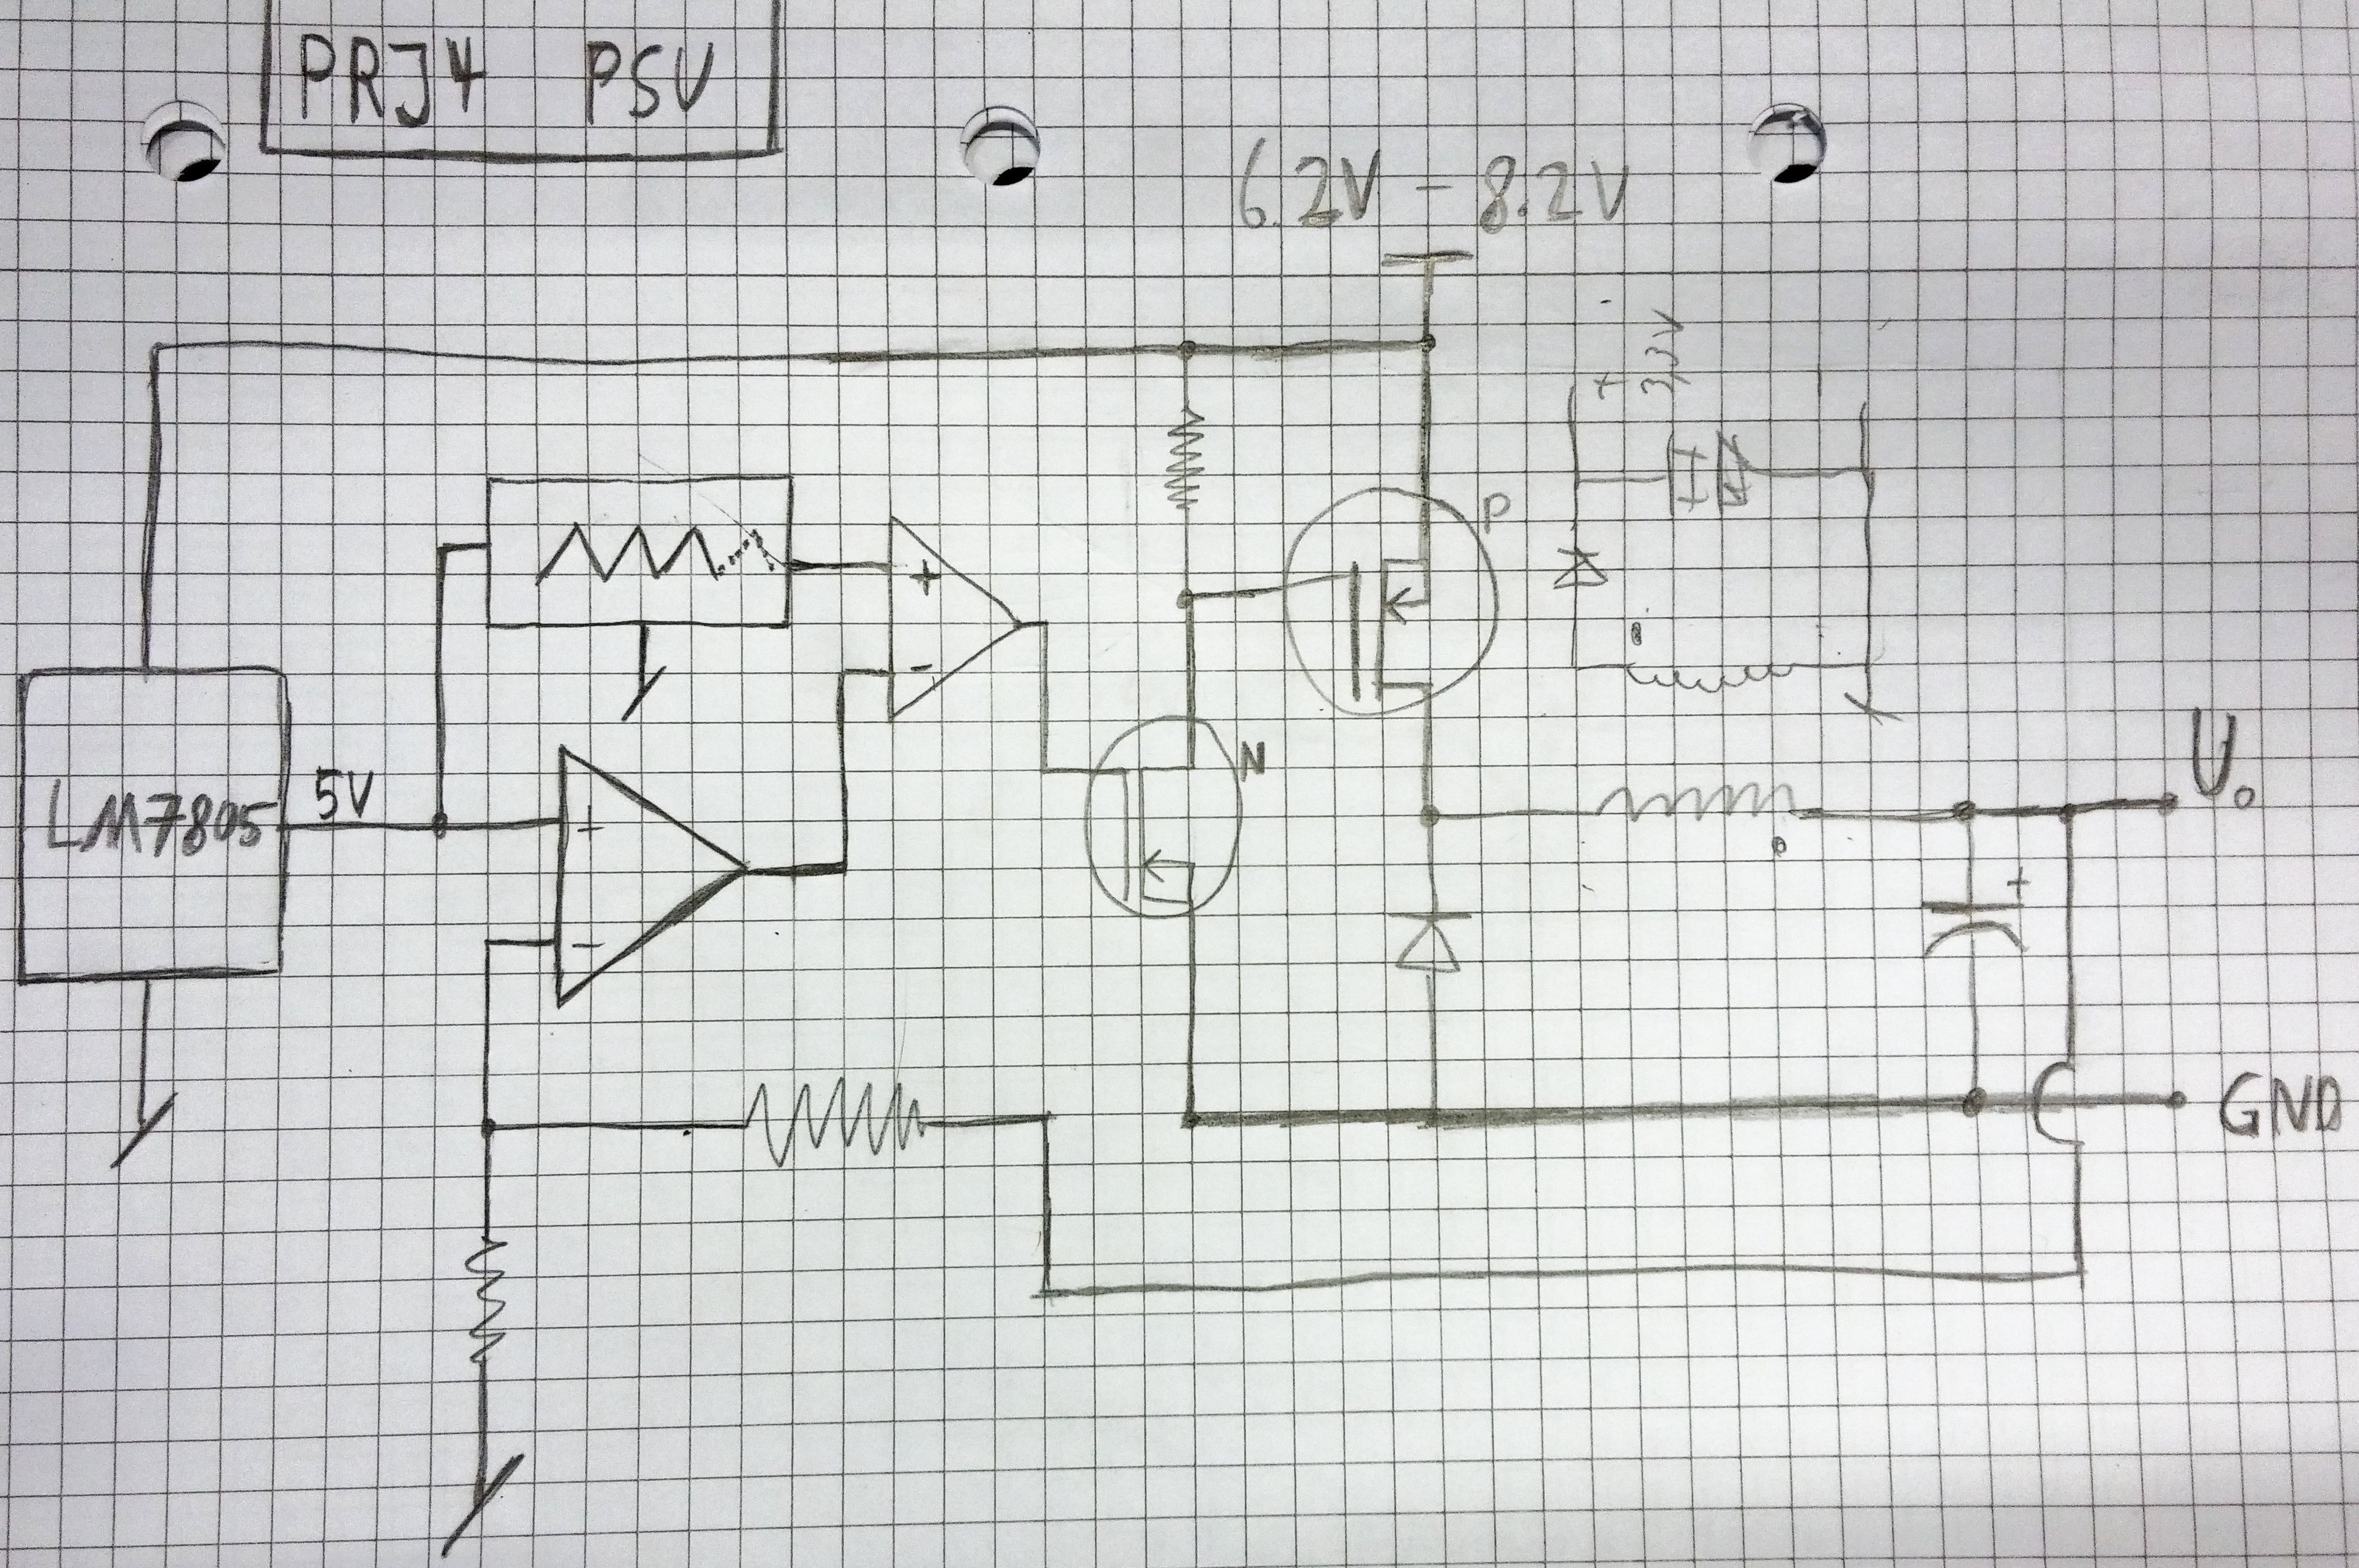
\includegraphics[width=\textwidth]{../fig/diagrammer/bil/psu_sketch}
\caption{Oprindelig tegning af bilens strømforsyning}
\label{fig:bil_psu_sketch}
\end{figure}

Som det kan ses i figur \ref{fig:bil_psu_sketch} var den oprindelige tanke at drive PWM signalet til switche ved hjælp af feedback fra udgangen, sammenlignet med den ønskede spænding, i dette tilfælde 5V, hvilket igen skulle sammenlignes med et trekantssignal for at give et firkantsignal med en pulsbredde på switchens indgang.
Det viste sig dog at være for kompliceret at realisere i det tidsomfang der var til rådighed og planen blev derfor skrottet.
Dog forefindes 3V udgangen, som er vist på højre side af diagrammet, stadig i det aktuelle design.

Det viste sig dog meget hurtigt at for at kunne opnå relativt kompakte kondensator- og spolestørrelser var det nødvendigt med et højfrekvent (100 kHz+) PWM signal til at drive switchen i strømforsyningen.
Der blev taget den beslutning i stedet at anvende en integreret løsning i form af Texas Instruments LM26003\cite{lib:lm26003}. 
Denne integrerede kreds samler fejlforstærkning, switch samt styring af clocksignal i ét.
Dette bringer størrelsen af strømforsyningen en del ned og giver højere effektivitet, da selve pakken for LM26003 ikke er større end ca 6 x 4 mm.
Dette blev vurderet til at være en fordel i designet og det blev også vurderet at en integreret kreds, som producenten garanterer for funktionaliteten af var fordelagtig ift. omfanget af projektet og hvor mange resourcer der kunne lægges i strømforsyningen kontra resten.

Da valget var truffet omkring LM26003'eren gik det næste ud på at finde ud af hvordan denne skulle kobles op optimalt og bruge de i databladet specificerede formler og metoder til at dimensionere det omkringliggende kredsløb.
Det endelige design kan ses i figur \ref{fig:bil_psu}.

\begin{figure}[h]
\centering
\includegraphics[width=\textwidth]{../fig/diagrammer/bil/psu_kredsloeb}
\caption{Det samlede diagram for bilens strømforsyning.}
\label{fig:bil_psu}
\end{figure}

Som udgangspunkt er de inderste viklinger dimensioneret ift. det antal $\mu H$ der er specificeret i udregningerne\cite{lib:psu_calcs} for strømforsyningen.
Der er herefter viklet et passende antal viklinger på for at generere et 3V firkantsignal, som derefter udrettes og filtreres.

På baggrund af den spoleform der er valgt har det været nødvendigt at designe egne komponenter i MutliSim og Ultiboard for at kunne realisere disse i et printudlæg senere.
